%!TEX root = ../BUSystematics.tex

\graphicspath{{Body/Figures/CBO/}{Body/Figures/CBO/Frequency/}{Body/Figures/CBO/TimeConstants/}}

% \clearpage
\section{CBO}


Beam dynamics terms, specifically relating to the radial coherent betatron oscillation (CBO), are included in the fits to the data. These terms account for the modulation that adjusts the observed $N$, $A$, and $\phi$ terms,
    \begin{align}
        N_{cbo}(t) &= N \cdot (1 + A_{cbo-N} \cdot e^{-t/\tau_{cbo}} \cdot \cos(\omega_{cbo}(t) \cdot t + \phi_{cbo-N})), \label{eq:Ncbo} \\ 
        A_{cbo}(t) &= A \cdot (1 + A_{cbo-A} \cdot e^{-t/\tau_{cbo}} \cdot \cos(\omega_{cbo}(t) \cdot t + \phi_{cbo-A})), \label{eq:Acbo} \\ 
        \phi_{cbo}(t) &= \phi_{0} + A_{cbo-\phi} \cdot e^{-t/\tau_{cbo}} \cdot \cos(\omega_{cbo}(t) \cdot t + \phi_{cbo-\phi}), \label{eq:Phicbo}
    \end{align}
where each CBO term has an amplitude, time constant, frequency, and phase associated with it. The frequency is time-dependent owing to the fact that the electrostatic quadrupoles were damaged during Run~1. The form for the frequency was determined from the tracking analysis and is given by
    \begin{align} \label{eq:CBOfreqForm}
        \omega_{cbo}(t) = \omega_{cbo} \cdot \Big(1 + \frac{Ae^{-t/\tau_{A}}}{\omega_{0}t} + \frac{Be^{-t/\tau_{B}}}{\omega_{0}t}\Big),
    \end{align}
where $\omega_{cbo}$ is the fit parameter and the rest of the parameters are fixed. The decoherence envelope is assumed to be an exponentially decaying cosine. Uncertainties in various pieces of the CBO model will contribute to systematic uncertainties on \R. More details on the construction and inclusion of the CBO in the fits can be found in \refref{phdthesis:2020Kinnaird}\footnote{Also included in fits to the data is a $N_{2-cbo}$ term at twice the CBO frequency.}.


\subsection{Frequency Model}

The fixed parameters in \equref{eq:CBOfreqForm} come from the tracking analysis \cite{CBOFreqTrackingElog}, and are shown in \figref{fig:CBOFreq} for the Endgame dataset. These parameters are determined separately for tracker stations 12 and 18, and by default the station 12 parameters are used in the fits. The systematic uncertainty was evaluated by using the tracker station 18 parameters, and taking the \DR as the systematic uncertainty. \tabref{tab:systematicError_CBOFreq} gives the systematic uncertainties for the four datasets and both fit methods. A less conservative approach which can be used in the future is to use the average of the station 12 and 18 parameters as the values in the fit, and then take as the systematic uncertainties the difference to either of the two stations.

% The HighKick and 9d Ratio results are less affected, presumably because the lifetime is fixed in those fits and there is a correlation.


\begin{figure}[h]
    \centering
    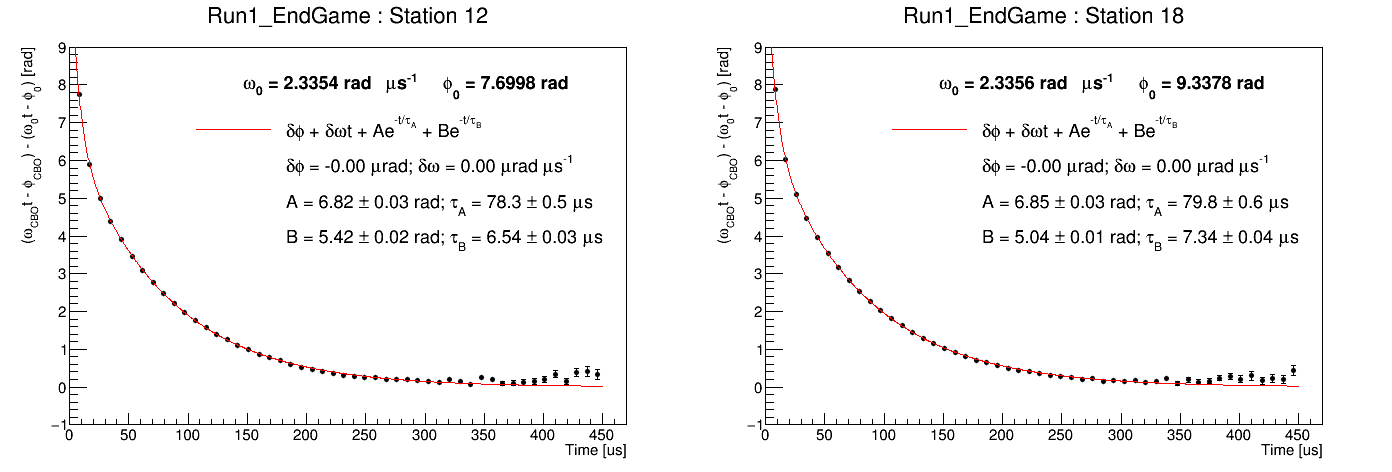
\includegraphics[width=\textwidth]{Run1_EndGame_CBOFreq}
    \caption[]{CBO frequency parameters for the Endgame dataset as determined in the tracking analysis for station 12 (left) and station 18 (right). The CBO frequency change is due to the slowly changing electrostatic quadrupole voltages over each fill. Plotted is the difference between the cosine argument for the changing frequency and the value it asymptotes to at late times. The frequency fit model includes two exponentials, one with a longer time constant and one with a shorter time constant. Plots courtesy of J. Mott.}
    \label{fig:CBOFreq}
\end{figure}


\begin{table}[h]
\centering
\renewcommand{\arraystretch}{1.2}
\begin{tabularx}{0.5\linewidth}{@{\extracolsep{\fill}}XYY}
  \hline
    \multicolumn{3}{c}{\textbf{CBO Frequency Systematic Uncertainty}} \\
  \hline\hline
    Dataset & \thead{T-Method} & \thead{R-Method} \\
  \hline
    60h & 10.9 & 5.3 \\
    HighKick & 22.5 & 0.7 \\
    9d & 21.3 & 1.6 \\ 
    Endgame & 22.2 & 8.5 \\
  \hline
\end{tabularx}
\caption[]{Systematic uncertainty due to the changing CBO frequency model. Units are in ppb.}
\label{tab:systematicError_CBOFreq}
\end{table}




% \clearpage
\subsection{Decoherence Envelope}


The decoherence envelope for the CBO was assumed to be a decaying exponential. The systematic uncertainty from the model was estimated by introducing a constant $C$ in the envelope,
    \begin{align}
        e^{-t/\tau_{cbo}} \rightarrow e^{-t/\tau_{cbo}} + C,
    \end{align}
which was motivated from the tracking analysis \cite{phdthesis:2020Kinnaird}. The constant $C$ was allowed to float in the fits, and the observed \DR values were then taken as the systematic uncertainties. \tabref{tab:CBOenvConstants} gives the fit results for the $C$ parameters and the associated errors. As shown the relative error on the parameter is typically around 50\% of the amplitude, with cases ranging from 30--90\%. In general the fits were perfectly happy with the additional fit parameter. \tabref{tab:systematicError_CBOenvelope} gives the systematic uncertainties for the different datasets and fit methods. As a quick note, this error was observed to vary significantly both among the different datasets and different analyzers, ranging in the low ppbs up to 40 or 50~ppb depending on the specific analysis. For this reason this systematic uncertainty was re-evaluated for the Endgame dataset at the final fit start time near \mus{50}, and these new numbers are included in both tables. While the fitted constant $C$ did not change significantly, the systematic uncertainty noticeably increased for the later fit start time.


\begin{table}[h]
\centering
\setlength\tabcolsep{10pt}
\renewcommand{\arraystretch}{1.2}
\begin{tabularx}{0.6\linewidth}{XYYY}
  \hline
    \multicolumn{4}{c}{\textbf{Fitted CBO Envelope Constants}} \\
  \hline\hline
    Dataset & \thead{Fit Method} & \multicolumn{1}{c}{$C$} & \multicolumn{1}{c}{$\delta C$} \\
  \hline
    \multirow{2}{*}{60h} & \thead{T} & 7.1 & 4.0 \\
                         & \thead{R} & 16.1 & 5.1 \\
  \hline
    \multirow{2}{*}{HighKick} & \thead{T} & 5.2 & 1.8 \\
                              & \thead{R} & 15.7 & 11.2 \\
  \hline
    \multirow{2}{*}{9d} & \thead{T} & 7.8 & 2.9 \\
                        & \thead{R} & 13.7 & 12.3 \\
  \hline
    \multirow{2}{*}{Endgame} & \thead{T} & 5.5 & 2.1 \\
                             & \thead{R} & 10.9 & 3.4 \\
  \hline
    \multirow{2}{*}{Endgame at \mus{50}} & \thead{T} & 4.7 & 2.6 \\
                                         & \thead{R} & 9.0 & 4.5 \\
  \hline  
\end{tabularx}
\caption[]{Fitted CBO envelope constants $C$ for each dataset and fit method. R-Method fits tended to have larger fitted $C$ parameters with larger errors, in accordance with the fact that the R-Method is less sensitive to the CBO effect after it is partially divided out. Units are in 1e-4.}
\label{tab:CBOenvConstants}
\end{table}





\begin{table}[h]
\centering
\renewcommand{\arraystretch}{1.2}
\begin{tabularx}{0.7\linewidth}{@{\extracolsep{\fill}}XYY}
  \hline
    \multicolumn{3}{c}{\textbf{CBO Decoherence Envelope Systematic Uncertainty}} \\
  \hline\hline
    Dataset & \thead{T-Method} & \thead{R-Method} \\
  \hline
    60h & 38.3 & 5.5 \\
    HighKick & 3.7 & 9.1 \\
    9d & 13.4 & 0.2 \\ 
    Endgame & 3.3 & 5.9 \\
    Endgame at \mus{50} & 25.3 & 18.0 \\
  \hline
\end{tabularx}
\caption[]{Systematic uncertainty due to the CBO decoherence envelope model. Units are in ppb.}
\label{tab:systematicError_CBOenvelope}
\end{table}



\clearpage
\subsection{Time Constants in CBO Terms}

As shown in Equations~\ref{eq:Ncbo}, \ref{eq:Acbo}, and \ref{eq:Phicbo}, each CBO term has the same CBO time constant by definition. Simulations showed however that these CBO time constants on the individual $A$ and $\phi$ terms could be as much as 50\% different from the time constant on the leading $N$ term. In order to evaluate a systematic uncertainty from this possibility, fits were redone by applying multipliers of 0.5 and 1.5 in the various combinations to the respective time constants, for a total of four new fits for each dataset. The maximum \DR seen from any of the combinations was then taken as the systematic uncertainty on \R. Tables~\ref{tab:systematicError_CBOtimeconstants_T} and \ref{tab:systematicError_CBOtimeconstants_R} show the results for the T- and R-Methods respectively. As shown, the combination of the multipliers 0.5 and 1.5 on the asymmetry and phase terms respectively almost always produced the largest differences.



\begin{table}[h]
\centering
\setlength\tabcolsep{15pt}
\renewcommand{\arraystretch}{1.2}
\begin{tabularx}{0.75\linewidth}{@{\extracolsep{\fill}}lGGGG}
  \hline
    \multicolumn{5}{c}{\textbf{T-Method \DR's with Multipliers on CBO Time Constants}} \\
  \hline\hline
    Dataset & \thead{(0.5, 0.5)} & \thead{(1.5, 0.5)} & \thead{(0.5, 1.5)} & \thead{(1.5, 1.5)} \\
  \hline
    60h & -6.3 & 8.6 & \multicolumn{1}{K}{-10.8} & 4.3 \\
    HighKick & -9.6 & \multicolumn{1}{K}{23.1} & -22.7 & 9.8 \\
    9d & 15.7 & -13.0 & \multicolumn{1}{K}{23.4} & -5.7 \\ 
    Endgame & -8.2 & 5.4 & \multicolumn{1}{K}{-10.5} & 3.2 \\
  \hline
\end{tabularx}
\caption[]{\DR's for the various multiplier combinations for the T-Method fits. Multipliers are on the asymmetry and phase CBO lifetime respectively. The absolute value of the bold elements are taken as the systematic uncertainties for the various datasets. Units are in ppb.}
\label{tab:systematicError_CBOtimeconstants_T}
\end{table}


\begin{table}[h]
\centering
\setlength\tabcolsep{15pt}
\renewcommand{\arraystretch}{1.2}
\begin{tabularx}{0.75\linewidth}{@{\extracolsep{\fill}}lGGGG}
  \hline
    \multicolumn{5}{c}{\textbf{R-Method \DR's with Multipliers on CBO Time Constants}} \\
  \hline\hline
    Dataset & \thead{(0.5, 0.5)} & \thead{(1.5, 0.5)} & \thead{(0.5, 1.5)} & \thead{(1.5, 1.5)} \\
  \hline
    60h & -0.1 & 9.3 & \multicolumn{1}{K}{-10.8} & -1.8 \\
    HighKick & -13.1 & 18.0 & \multicolumn{1}{K}{-21.8} & 9.3 \\
    9d & -2.4 & -28.7 & \multicolumn{1}{K}{30.9} & 3.3 \\ 
    Endgame & -6.9 & 5.0 & \multicolumn{1}{K}{-9.8} & 2.3 \\
  \hline
\end{tabularx}
\caption[]{\DR's for the various multiplier combinations for the R-Method fits. Multipliers are on the asymmetry and phase CBO lifetime respectively. The absolute value of the bold elements are taken as the systematic uncertainties for the various datasets. Units are in ppb.}
\label{tab:systematicError_CBOtimeconstants_R}
\end{table}





\clearpage
\subsection{Fixed Time Constants in the R-Method}

In the HighKick and 9d datasets, the CBO time constants in the R-Method fits were fixed to those values determined from corresponding T-Method fits. This was done because otherwise the fits did not converge properly. Parameters which float in the fit contribute to the statistical uncertainty, but parameters which are fixed contribute to a systematic uncertainty, since it's possible the parameter should have been fixed to a value other than that which was chosen\footnote{Since the CBO time constant was allowed to float in the 60h and Endgame datasets, no such systematic uncertainty exists for those datasets.}. The systematic uncertainty for the HighKick and 9d datasets were evaluated in the usual way by determining the sensitivity of \R to the time constant parameter, and multiplying it against the corresponding uncertainty in the time constant. The former was determined by scanning over a range of fixed values about the T-Method value, and the latter was taken from the statistical uncertainty in the parameter as determined in the T-Method fit. \figref{fig:CBOfixedLifetime} shows the scan results for the HighKick and 9d datasets. The corresponding sensitivities and systematic uncertainties are shown in \tabref{tab:systematicError_FixedCBOLifetime}. As shown the systematic uncertainties are almost negligible at a few ppb or less.



\begin{figure}[h]
\centering
    \begin{subfigure}[t]{0.45\textwidth}
        \centering
        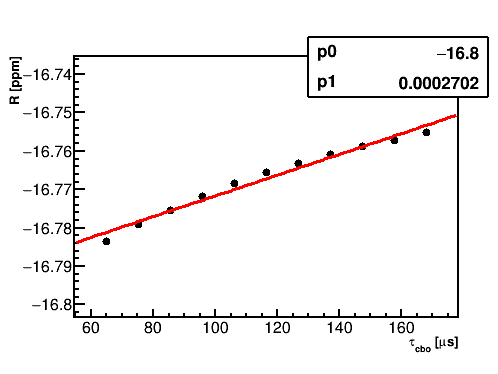
\includegraphics[width=\textwidth]{FullRatio_R_Vs_tau_cbo_Canv_HK}
        \caption{HighKick dataset.}
    \end{subfigure}% %you need this % here to add spacing between subfigures
    \hspace{1cm}
    \begin{subfigure}[t]{0.45\textwidth}
        \centering
        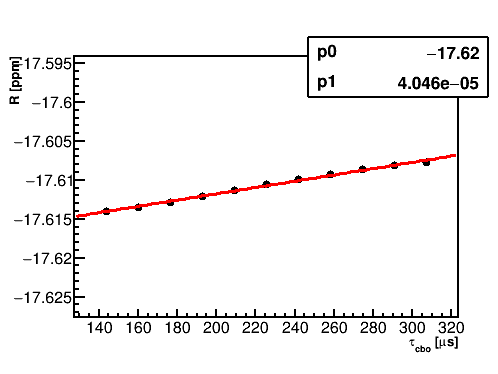
\includegraphics[width=\textwidth]{FullRatio_R_Vs_tau_cbo_Canv_9d}
        \caption{9d dataset.}
    \end{subfigure}
\caption[]{\R vs fixed CBO time constant for the HighKick and 9d datasets. The parameter $p_{1}$ is in units of ppm per microsecond. There is a wavy structure in the points, but the effect is sub-leading and therefore ignored.}
\label{fig:CBOfixedLifetime}
\end{figure}


\begin{table}[h]
\centering
\renewcommand{\arraystretch}{1.2}
\begin{tabularx}{0.65\linewidth}{@{\extracolsep{\fill}}XccY}
  \hline
    \multicolumn{4}{c}{\textbf{Fixed CBO Time Constant Systematic Uncertainty}} \\
  \hline\hline
    Dataset & \thead{$dR/d\tau_{cbo}$} & \thead{T-Method $\sigma_{\tau_{cbo}}$} & \thead{R-Method \dR} \\
  \hline
    HighKick & 0.27 & 10.3 & 2.8 \\
    9d & 0.04 & 16.3 & 0.7 \\ 
  \hline
\end{tabularx}
\caption[]{Systematic uncertainty due to fixed CBO time constants in the HighKick and 9d datasets. Units are in ppb per microsecond for the sensitivity, microsecond for the uncertainty, and ppb for the systematic uncertainty.}
\label{tab:systematicError_FixedCBOLifetime}
\end{table}
